% Los fragmentos de SystemVerilog y los rangos de buses emplean comillas,
% paréntesis y guiones con una semántica distinta de la prosa.
% chktex-file 1
% chktex-file 8
% chktex-file 18
% chktex-file 36

\section{El problema de las entradas manuales}

La ALU puede describirse sin reloj, pero utilizarla desde la placa
introduce un problema adicional. Los pulsadores cambian cuando el
usuario los acciona y, por lo tanto, sus transiciones no guardan
relación con el reloj de \SI{100}{\mega\hertz}. Si una de ellas
ocurre cerca de un flanco, el primer registro que la recibe puede
entrar temporalmente en metastabilidad.

El módulo \texttt{button\_input} reduce el riesgo de que ese estado
se propague mediante dos flip-flops en serie. La primera etapa
captura el pin y dispone de casi un ciclo para estabilizarse; la
segunda recién utiliza esa muestra en el flanco siguiente.

\begin{codebox}[language=SystemVerilog]
  (* ASYNC_REG = "TRUE" *) reg button_meta = 1'b0;
  (* ASYNC_REG = "TRUE" *) reg button_sync = 1'b0;

  always @(posedge clk) begin
  button_meta <= button;
  button_sync <= button_meta;
  end

  assign button_pressed = button_sync;
\end{codebox}

Las asignaciones no bloqueantes son esenciales: ambos flip-flops
calculan su próximo estado a partir de los valores anteriores al
flanco. La segunda etapa no recibe inmediatamente la muestra nueva de
la primera. El atributo \texttt{ASYNC\_REG} informa a \tech{Vivado}
que ambos registros forman un sincronizador y permite que la
herramienta preserve esa relación durante la implementación.

La figura~\ref{fig:button-rtl} muestra la conexión que resulta de la
descripción. Esta estructura sincroniza un nivel, pero no elimina
rebotes ni genera un pulso de un solo ciclo. Esa diferencia determina
el modo de uso: los switches deben permanecer estables mientras el
botón está presionado y hasta que su liberación haya atravesado las dos etapas.

\begin{figure}[H]
  \centering
  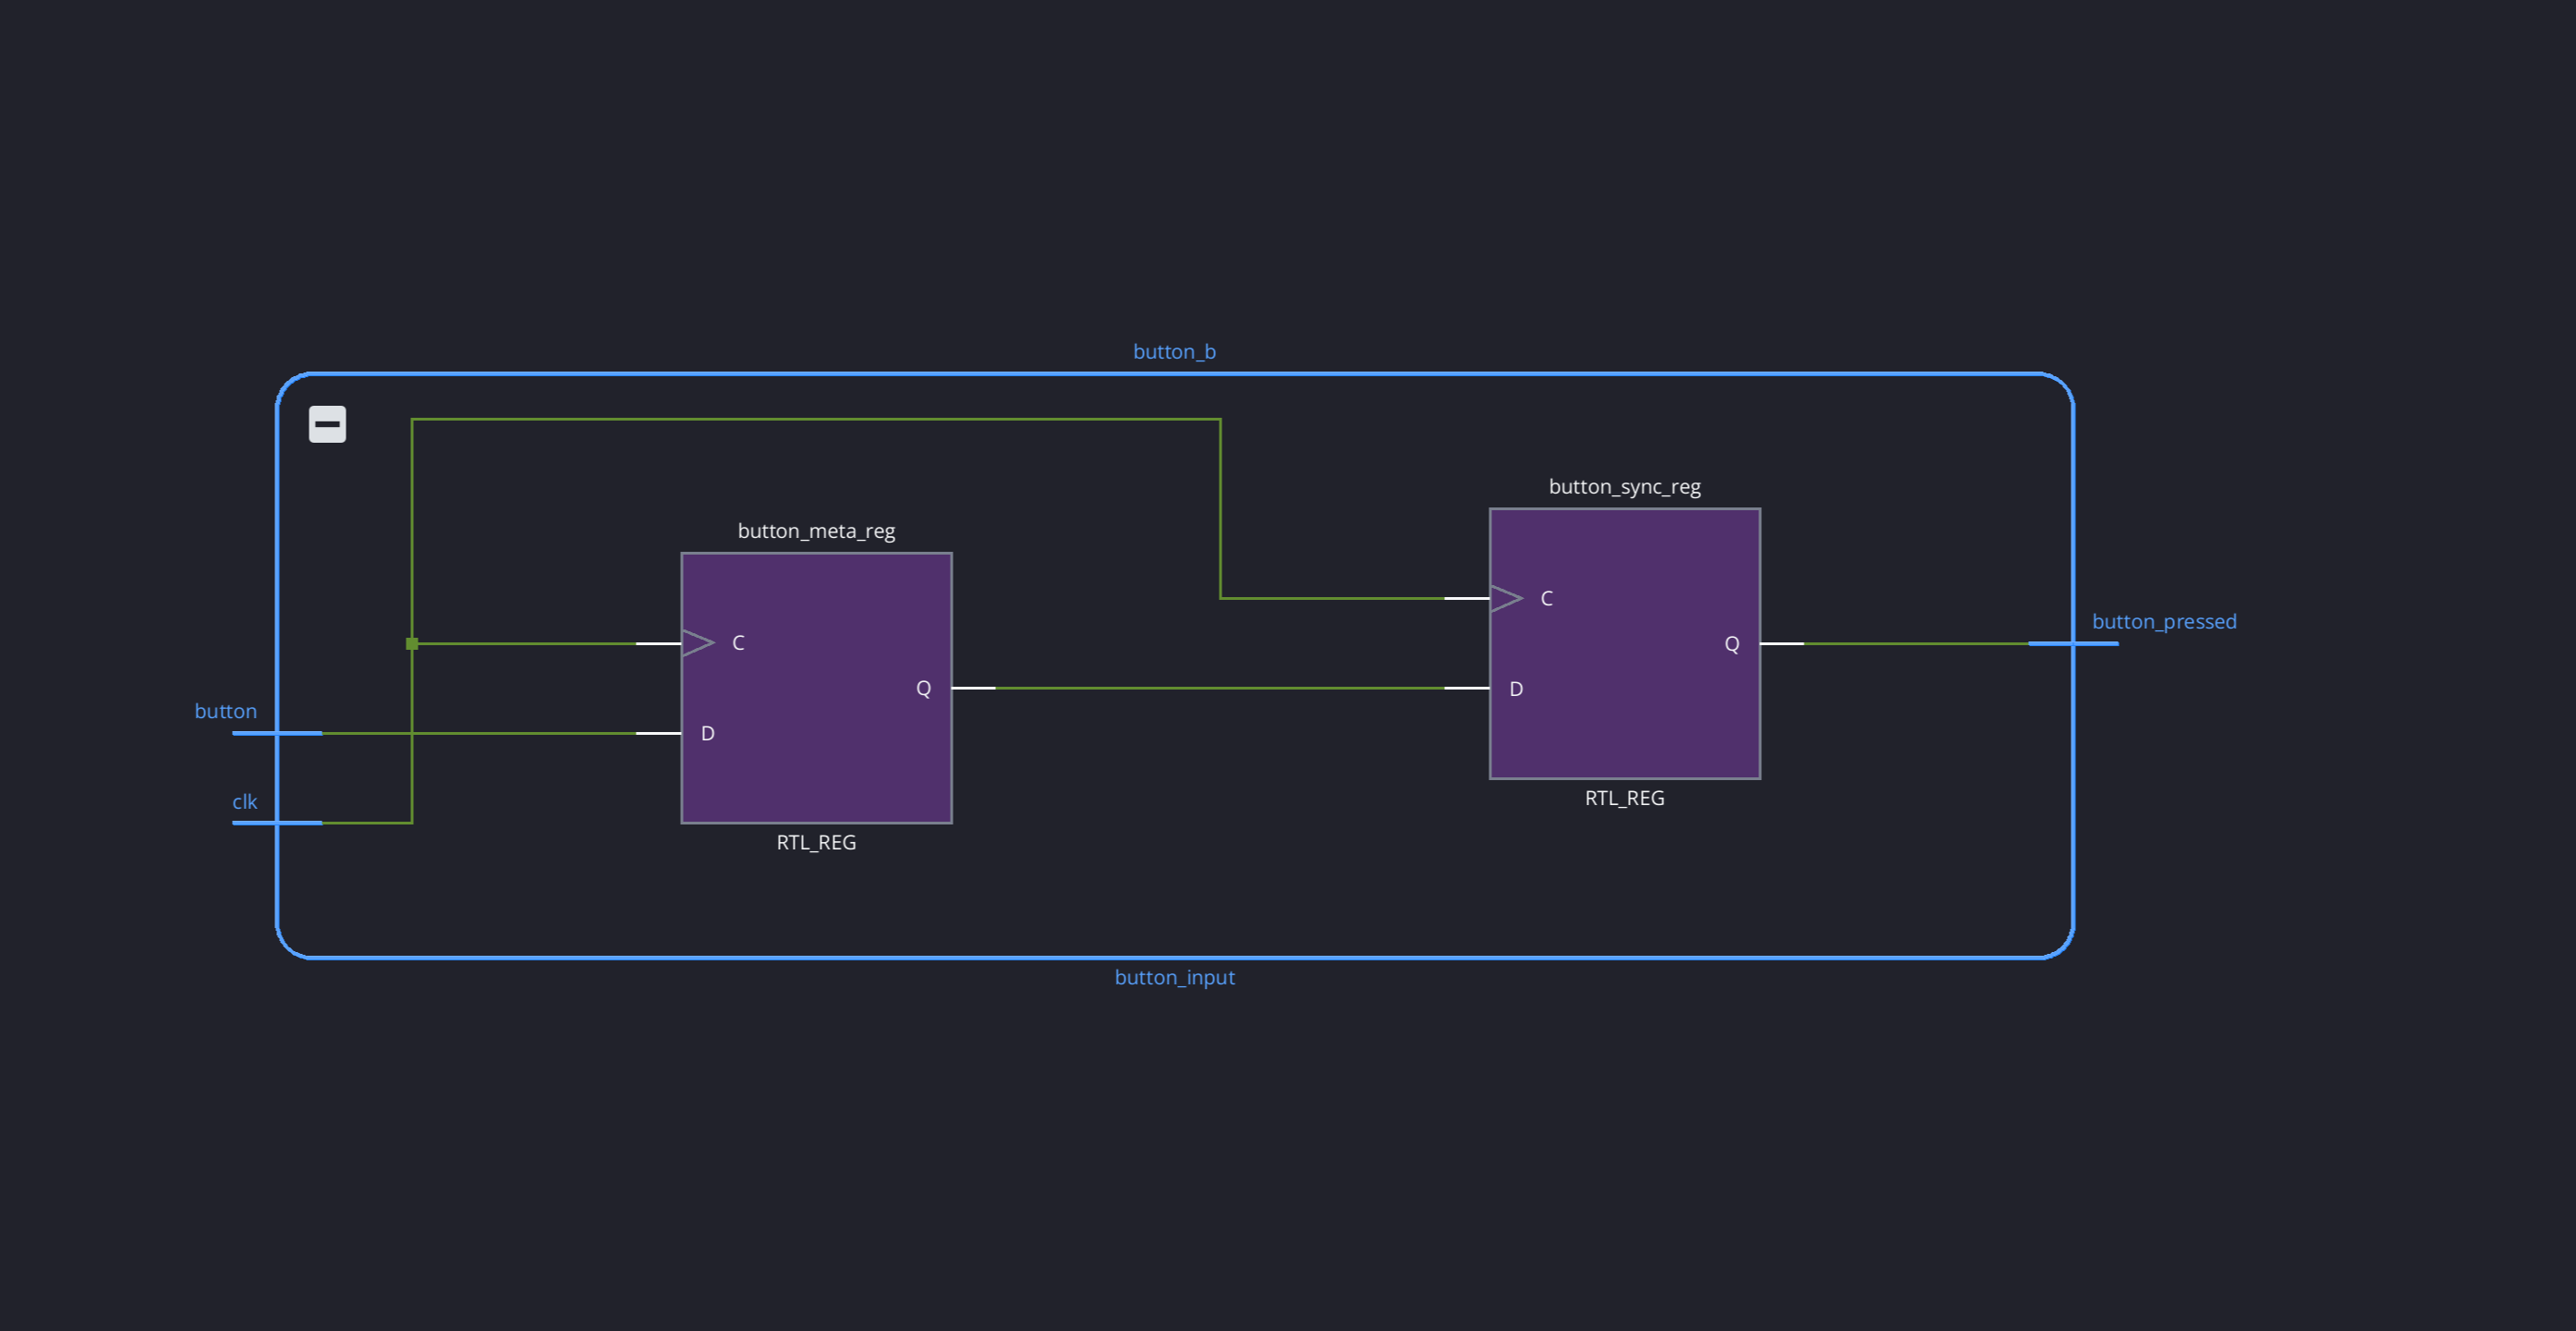
\includegraphics[width=\textwidth]{img/schematic_button_rtl.png}
  \caption{Cadena de dos registros utilizada para sincronizar un pulsador.}%
  \label{fig:button-rtl}
\end{figure}

\section{Registros de entrada y reset}

Una vez dentro del dominio del reloj, las señales de control sirven
como habilitaciones de \texttt{alu\_top}. A y B ocupan ocho bits y el
opcode utiliza los seis switches inferiores. Cada registro conserva
su contenido mientras su habilitación permanece inactiva.

El reset tiene prioridad sobre las tres cargas. La señal
\texttt{startup\_reset}, que comienza en uno, complementa al botón
central sincronizado y garantiza que los registros se borren en el
primer flanco posterior a la configuración.

\begin{codebox}[language=SystemVerilog]
  reg startup_reset = 1'b1;

  always @(posedge clk) begin
  startup_reset <= 1'b0;

  if (startup_reset || reset_pressed) begin
  data_a <= 8'b0;
  data_b <= 8'b0;
  opcode <= 6'b0;
  end else begin
  if (load_a)      data_a <= switches;
  if (load_b)      data_b <= switches;
  if (load_opcode) opcode <= switches[5:0];
  end
  end
\end{codebox}

Durante el primer flanco, el \texttt{if} todavía observa el valor
inicial de \texttt{startup\_reset}; su actualización a cero se aplica
al finalizar el paso. En ciclos posteriores decide el pulsador
central. Como las cargas se evalúan con tres condiciones
independientes, es posible cargar A y B simultáneamente con el mismo valor.

La vista RTL del módulo superior reúne estas piezas en la
figura~\ref{fig:top-rtl}. Allí, los sincronizadores llegan a las
habilitaciones de los registros y el bus de switches alimenta sus
entradas. Las salidas registradas se dirigen al núcleo combinacional,
del que parten los once bits conectados a los LEDs.

\begin{figure}[H]
  \centering
  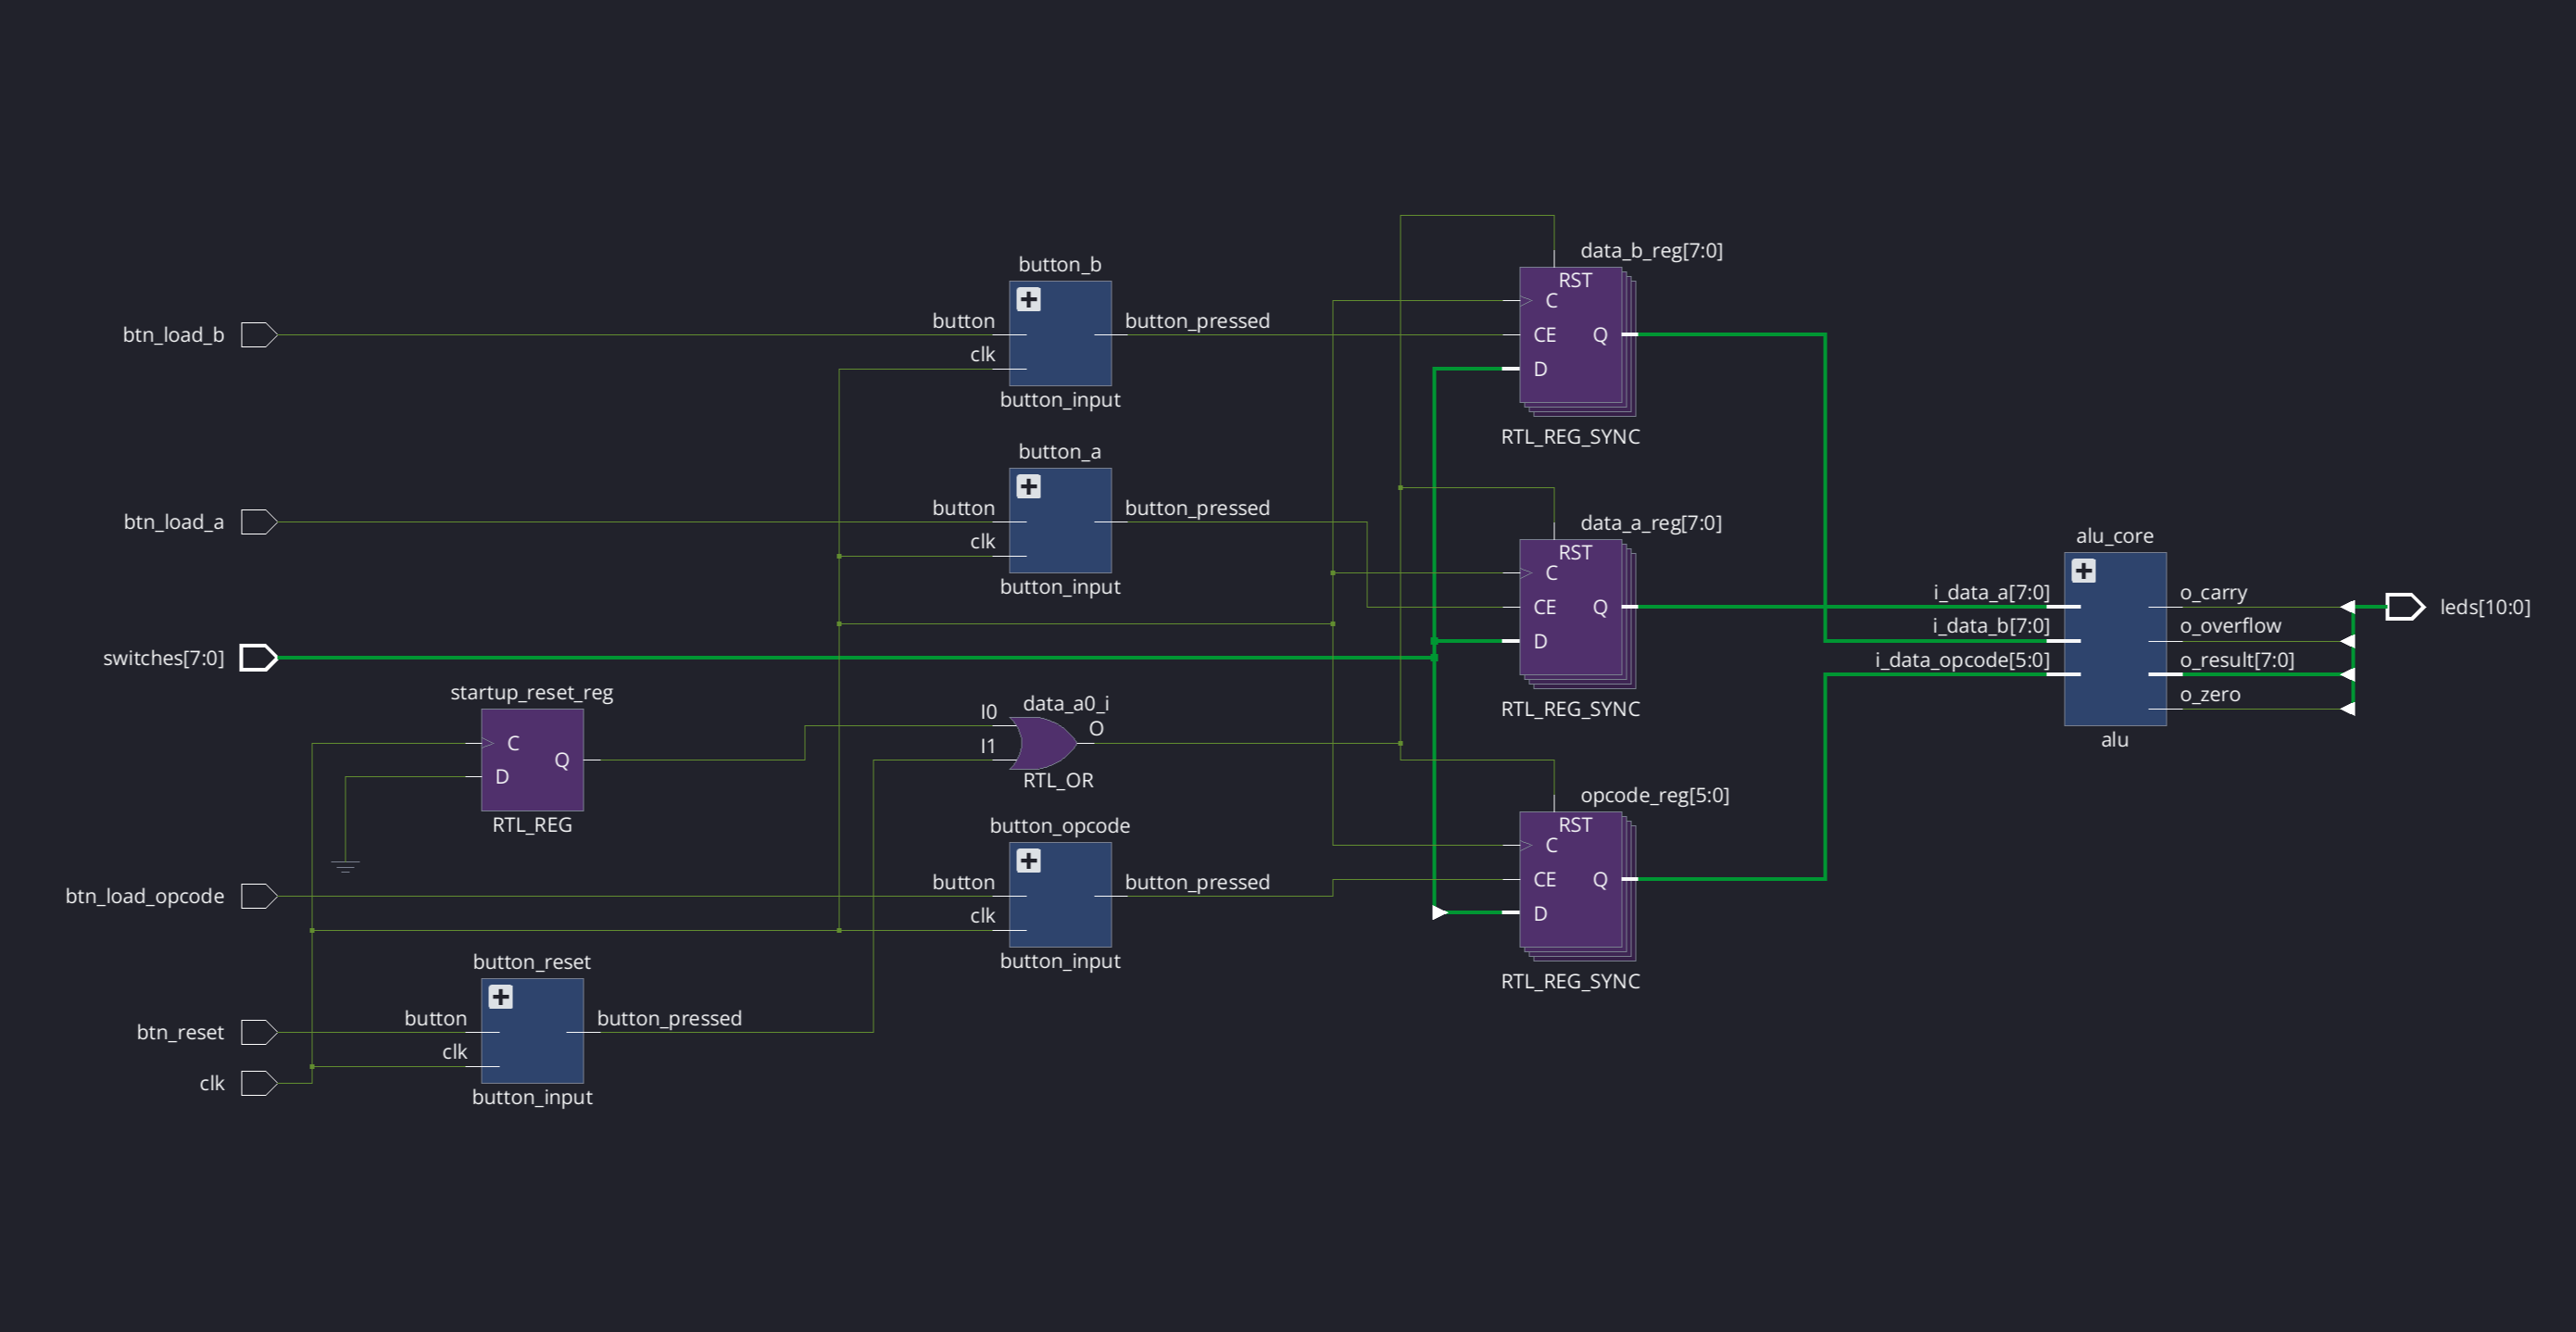
\includegraphics[width=\textwidth]{img/schematic_top_rtl.png}
  \caption{Integración de sincronizadores, registros y núcleo de la ALU.}%
  \label{fig:top-rtl}
\end{figure}

\section{Distribución de controles e indicadores}

La ubicación de los botones acompaña la secuencia de carga. BTNL
guarda A, BTNR guarda B y BTNU guarda el opcode. BTNC restablece el
estado inicial. El botón inferior queda libre.

\begin{table}[H]
  \centering
  \begin{tabularx}{\textwidth}{L{3.0cm}L{3.5cm}Y}
    \toprule
    \textbf{Recurso} & \textbf{Puerto} & \textbf{Función} \\
    \midrule
    SW7--SW0 & \texttt{switches[7:0]} & Dato compartido para las cargas. \\
    BTNL & \texttt{btn\_load\_a} & Cargar A. \\
    BTNR & \texttt{btn\_load\_b} & Cargar B. \\
    BTNU & \texttt{btn\_load\_opcode} & Cargar opcode desde SW5--SW0. \\
    BTNC & \texttt{btn\_reset} & Borrar A, B y opcode. \\
    LED7--LED0 & \texttt{leds[7:0]} & Resultado de ocho bits. \\
    LED8 & \texttt{leds[8]} & Indicador Z. \\
    LED9 & \texttt{leds[9]} & Indicador C. \\
    LED10 & \texttt{leds[10]} & Indicador V. \\
    \bottomrule
  \end{tabularx}
  \caption{Asignación funcional de los recursos de la Basys 3.}
\end{table}

Para calcular $5+3$, por ejemplo, se coloca \texttt{00000101} y se
utiliza BTNL para almacenarlo. A continuación, se utiliza BTNR para
cargar el valor \texttt{00000011}. Por último, se configura
\texttt{100000} en SW5--SW0 y se utiliza BTNU para guardar el opcode.
Los registros contienen entonces las tres entradas de ADD y LED3 se
enciende para representar \texttt{00001000}. Al pulsar BTNC, los
registros vuelven a cero y LED8 indica el resultado nulo.

\section{Conexiones físicas y restricciones}

El archivo \texttt{basys3.xdc} relaciona la interfaz funcional con
los pines de la placa. El reloj ingresa por W5 y se declara con un
período de \SI{10}{\nano\second}. Los pulsadores de A, B, opcode y
reset se conectan a W19, T17, T18 y U18. El resultado ocupa LED0 a
LED7, mientras que Z, C y V se asignan a LED8, LED9 y LED10.

La figura~\ref{fig:ports} reúne los 24 bits de entrada o salida y
permite revisar tanto el pin físico como el estándar \tech{LVCMOS33}.

\begin{figure}[H]
  \centering
  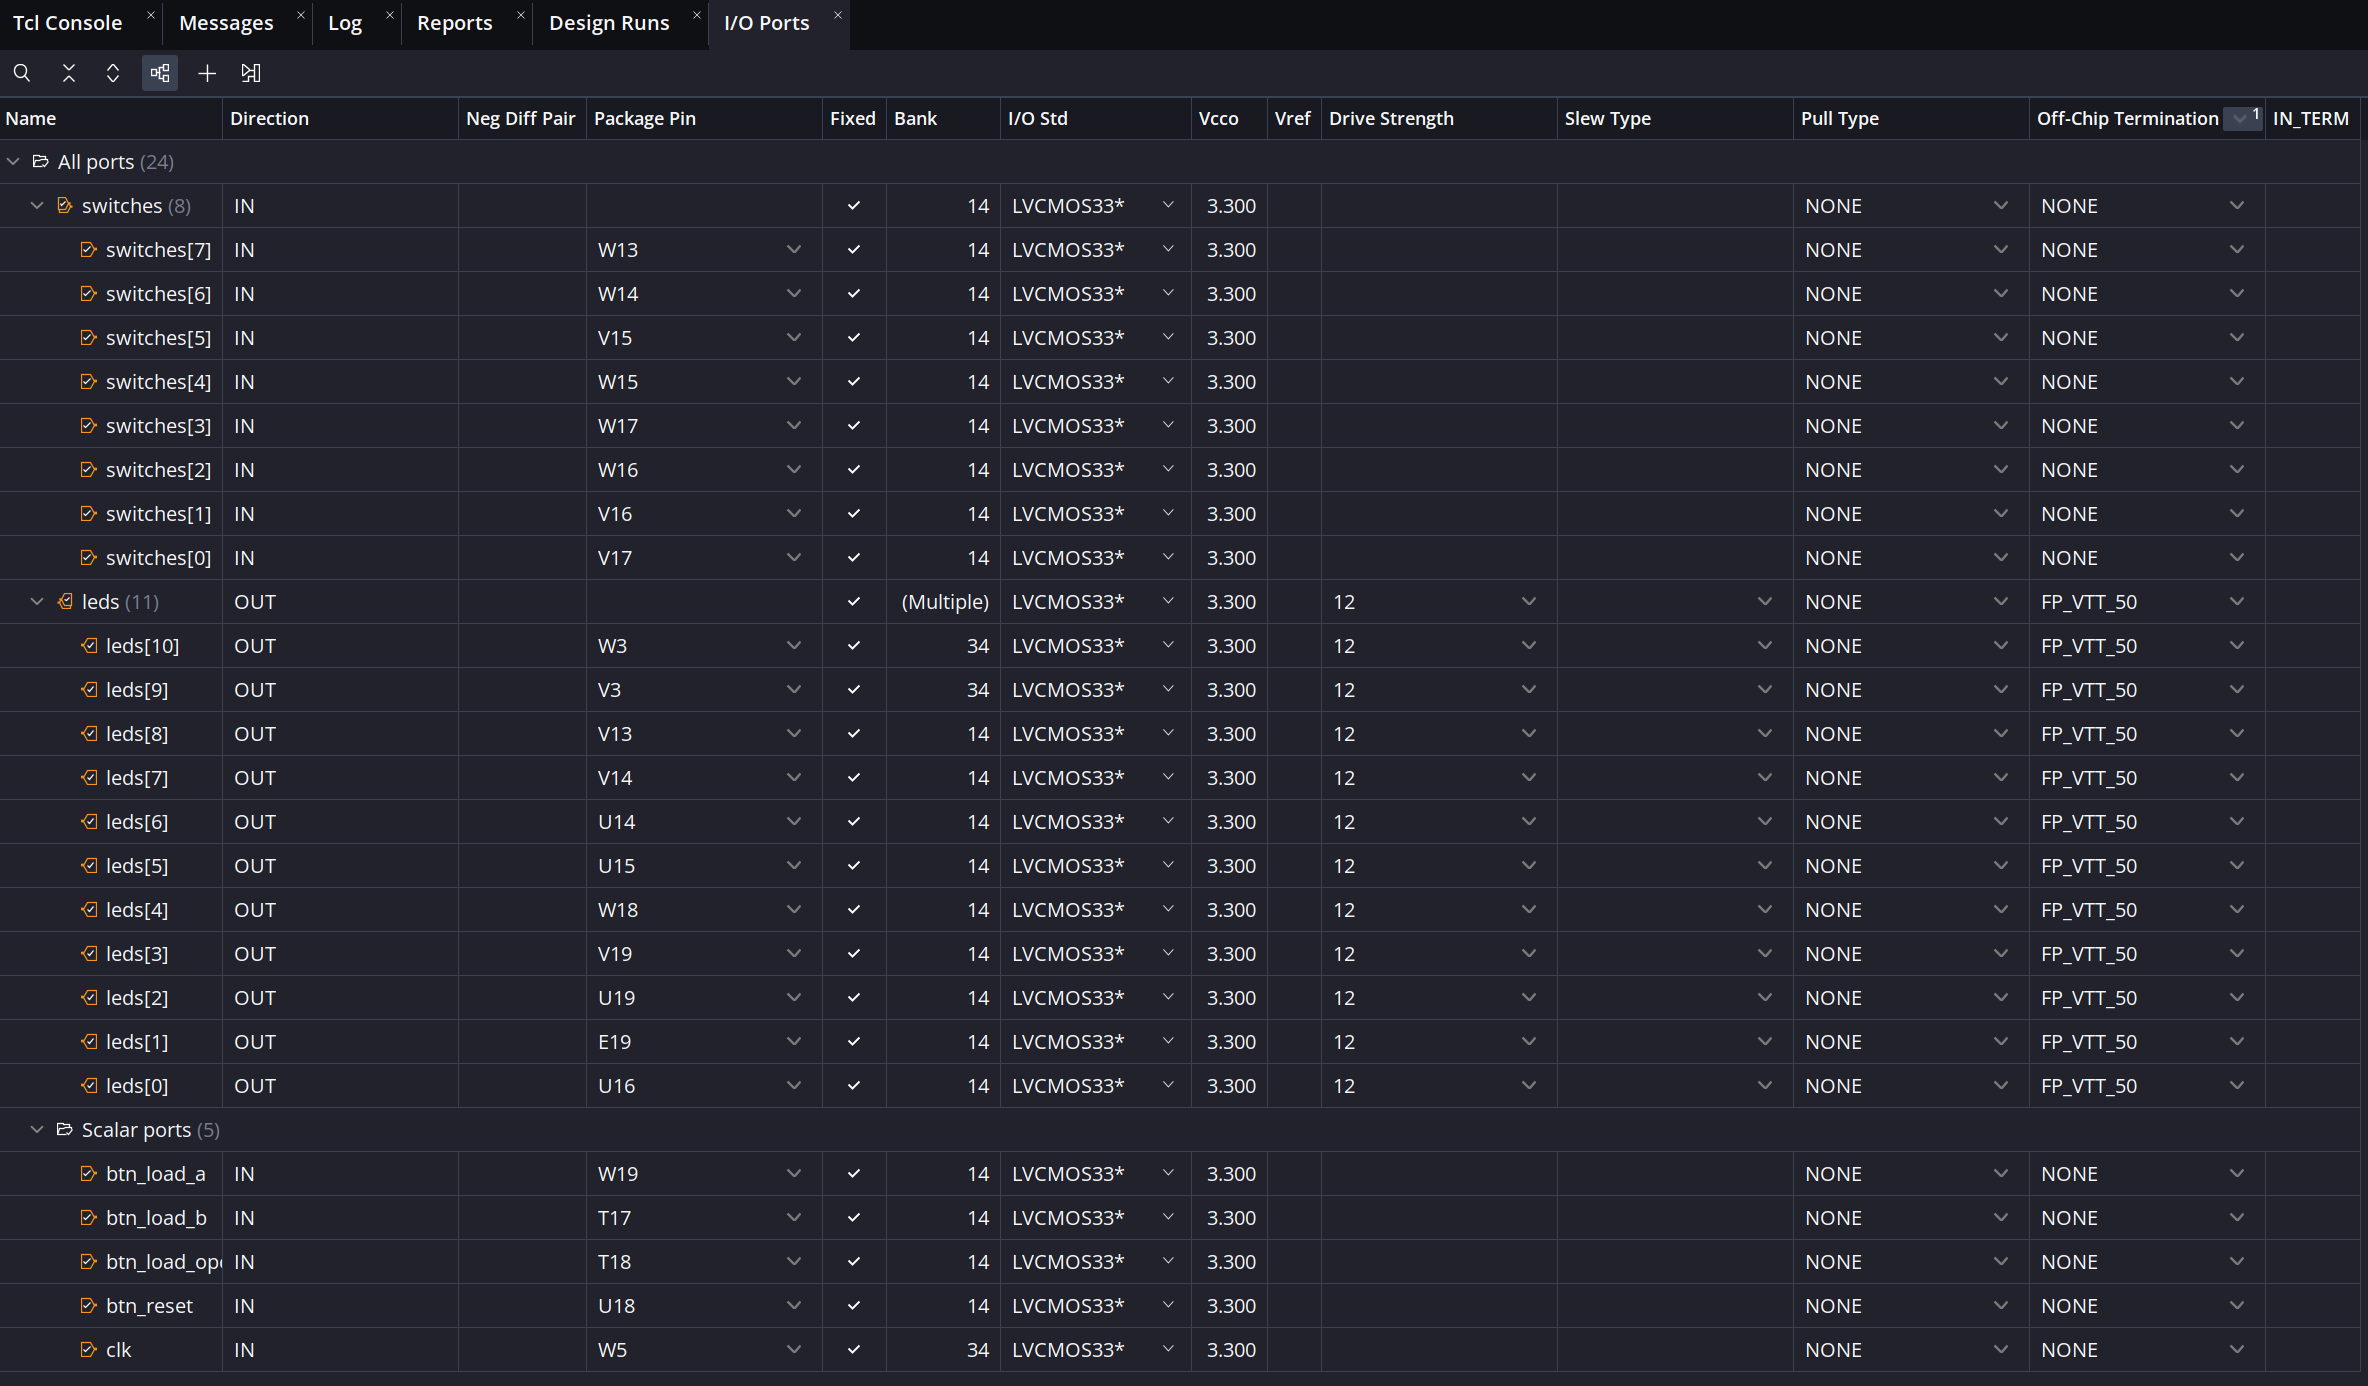
\includegraphics[width=\textwidth]{img/ports.png}
  \caption{Asignación de puertos, pines y estándar eléctrico.}%
  \label{fig:ports}
\end{figure}

Las restricciones temporales también documentan supuestos del
entorno. Los pulsadores se consideran asíncronos hasta la primera
etapa del sincronizador. Los switches se exceptúan porque el
procedimiento exige configurarlos antes de la carga, y los LEDs no
poseen un reloj externo que defina un instante de captura. Las rutas
internas entre registros continúan sujetas al reloj de la placa.

Esta distinción impide atribuir al reporte temporal más alcance del
que realmente tiene: un timing interno correcto no comprueba que el
usuario haya mantenido estable el bus ni mide el retardo
combinacional hasta uno de los LEDs.
